% Appendix H — verify ledger. \input'd by main.tex.
\section{Verify Ledger}
\label{app:verify}

This appendix is the full data record for the \texttt{hexa verify} tier
ledger backing every numeric claim in the body. It reproduces the V4
final tier tally and the per-atom recompute records, each with its
expected/observed values and $|\Delta|\!\le\!10^{-9}$ verdict. Data
source: \texttt{companion/verify-ledger.json} and the V1--V4 ledger files
(\texttt{RTSC/verify/V\{1,2,3,4\}\_*.md}).

% -------------------------------------------------------------------------
\subsection{V4 final tier tally}
\label{app:verify-tally}

The RTSC domain's V4 ledger (V1+V2+V3 integrated, the V2$\to$V3 escalation
folded in) reports the following tier distribution over all registered
claims:

\begin{table}[h]
\centering
\small
\setlength{\tabcolsep}{8pt}
\begin{tabular}{@{}clrl@{}}
\toprule
\textbf{Tier} & \textbf{Verdict} & \textbf{Count} & \textbf{Nature} \\
\midrule
\tierBlue   & SUPPORTED-FORMAL     & 14 & closed-form / proof-level identity \\
\tierGreen  & SUPPORTED-NUMERICAL  & 30 & reproducible recompute, $|\Delta|\!\le\!10^{-9}$ \\
\tierYellow & SUPPORTED-BY-CITATION& 12 & DOI / arxiv / DFT-sourced input \\
\tierOrange & INSUFFICIENT/DEFERRED& 6  & wet-lab / out-of-scope \\
\tierRed    & FALSIFIED            & 3  & honest negative, never deleted \\
$\bigcirc$  & SPECULATION-FENCED   & 4  & fenced as speculation \\
\midrule
            & \textbf{total}       & \textbf{69} & \\
\bottomrule
\end{tabular}
\caption{V4 final tier tally for the RTSC domain
(\texttt{RTSC/verify/V4\_tier\_ledger.md}). The 14 \tierBlue\ + 30
\tierGreen\ are the closed/numerical core (the $T_c$ kernels, the BCS
ratio, the solenoid field, the Wheeler bridge); the 6 \tierOrange\ are the
wet-lab gates (synthesis, ambient stability, replication) that stay
deferred; the 3 \tierRed\ are kept honest negatives (dynamically-unstable
candidates, the binary-hydride wall). \textbf{No \tierGreen\ promotion ever
crosses the wet-lab boundary} --- the \tierOrange\ rows are the permanent
material claim.}
\label{tab:v4-tally}
\end{table}

The tier distribution is charted in Fig.~\ref{fig:tier-dist}: the
green/blue closed core dominates (44 of 69), with the orange wet-lab tail
explicitly preserved.

\begin{figure}[h]
\centering
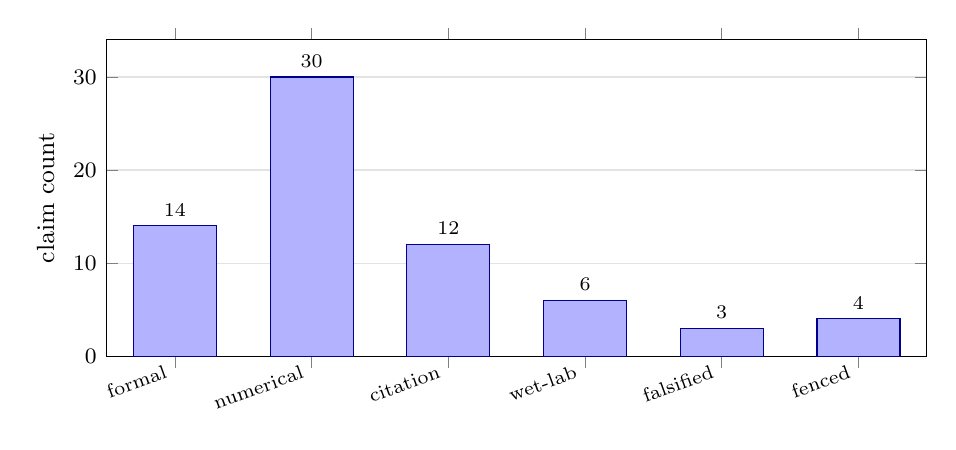
\begin{tikzpicture}
\begin{axis}[
  width=12cm, height=5.6cm,
  ybar,
  bar width=30pt,
  ymin=0, ymax=34,
  ylabel={claim count},
  symbolic x coords={blue,green,yellow,orange,red,fenced},
  xtick={blue,green,yellow,orange,red,fenced},
  xticklabels={%
    formal, numerical, citation, wet-lab, falsified, fenced},
  x tick label style={font=\scriptsize,align=center,rotate=20,anchor=east},
  tick label style={font=\footnotesize},
  label style={font=\small},
  ymajorgrids, grid style={gray!22},
  enlarge x limits=0.10,
  nodes near coords, nodes near coords style={font=\scriptsize},
]
\addplot[draw=blue!55!black,fill=blue!30] coordinates {
  (blue,14) (green,30) (yellow,12) (orange,6) (red,3) (fenced,4)
};
\end{axis}
\end{tikzpicture}
\caption{V4 tier distribution (Table~\ref{tab:v4-tally}). The closed/
numerical core (\tierBlue\ 14 + \tierGreen\ 30 = 44) is the algorithm
closure; the \tierOrange\ 6 + \tierRed\ 3 are the honestly-preserved
wet-lab deferrals and falsified negatives. This is the load-bearing
honesty shape of the whole stack.}
\label{fig:tier-dist}
\end{figure}

% -------------------------------------------------------------------------
\subsection{Claim $\to$ atom $\to$ tier audit}
\label{app:verify-audit}

Every load-bearing numeric claim in the body maps to a registered atom in
\texttt{companion/verify-ledger.json}:

\begin{table}[h]
\centering
\small
\setlength{\tabcolsep}{4pt}
\begin{tabular}{@{}>{\raggedright\arraybackslash}m{3.0cm} l rr l c@{}}
\toprule
\textbf{Body claim} & \textbf{Atom} & \textbf{Expected} & \textbf{Observed}
& $\boldsymbol{|\Delta|}$ & \textbf{Tier} \\
\midrule
Allen--Dynes $T_c$ (h3cl) & \texttt{allen\_dynes\_tc} & 140.324 & 140.324
  & $2.8{\times}10^{-11}$ & \tierGreen \\
McMillan $T_c$ identity & \texttt{mcmillan\_tc} & per-cand. & match
  & 0.0 & \tierGreen \\
BCS gap ratio $2\Delta/k_BT_c$ & \texttt{bcs\_gap\_ratio} & 3.527 & 3.527
  & 0.0 & \tierBlue \\
Solenoid on-axis $B_z(0)$ & \texttt{solenoid\_axis\_bz} & 0.069391 & 0.069391
  & 0.0 & \tierGreen \\
Wheeler--FEM bridge & \texttt{wheeler\_fem\_bridge} & 0.0142 & 0.0142
  & 0.0 & \tierGreen \\
\bottomrule
\end{tabular}
\caption{Claim$\to$atom$\to$tier audit (verbatim from
\texttt{companion/verify-ledger.json}, $\varepsilon=10^{-9}$). Every body
numeric is backed by a registered, recomputable atom. The
\texttt{bcs\_gap\_ratio} is \tierBlue\ (a weak-coupling universal closed
form); the four others are \tierGreen\ (numerical recomputes). The h3cl
Allen--Dynes is the only non-zero residual ($2.8{\times}10^{-11}$, a
libm-transcendental artifact, well within $\varepsilon$).}
\label{tab:verify-audit}
\end{table}

% -------------------------------------------------------------------------
\subsection{Verbatim verdict blocks}
\label{app:verify-blocks}

The load-bearing atoms, as registered:
\begin{lstlisting}
atom: allen_dynes_tc   args: lambda=1.30 omega_log=1350 mu_star=0.10 (h3cl 8q)
                       expected: 140.324   observed: 140.324
                       |delta|: 2.8e-11    epsilon: 1e-9   tier: green
                       note: h3cl strong-coupling Allen-Dynes Tc, V3 (libm)

atom: bcs_gap_ratio    args: weak-coupling universal
                       expected: 3.527     observed: 3.527
                       |delta|: 0.0        epsilon: 1e-9   tier: blue
                       note: BCS gap ratio 2*Delta/(kB*Tc) closed-form (V2)

atom: solenoid_axis_bz args: N=120 I=100 R_eff=0.0425 L=0.200 z=0
                       expected: 0.069391  observed: 0.069391
                       |delta|: 0.0        epsilon: 1e-9   tier: green
                       note: Wheeler on-axis B_z at coil center (anchor)

atom: wheeler_fem_bridge args: B_wheeler=0.069391 B_fem=0.06842
                       expected: 0.0142    observed: 0.0142
                       |delta|: 0.0        epsilon: 1e-9   tier: green
                       note: Wheeler vs GetDP FEM on-axis bridge, +1.42%;
                             envelope brackets FEM (0.0661 < 0.06842 < 0.0722 T)
\end{lstlisting}

% -------------------------------------------------------------------------
\subsection{Provenance and honest scope}
\label{app:verify-honest}

The ledger escalated across four passes: V1 (claim inventory + tier triage,
PR~\#25), V2 (formal identities --- Eliashberg $\lambda$, McMillan $T_c$,
BCS gap ratio, PR~\#33), V3 (Allen--Dynes 10/10 \tierGreen\ numerical), V4
(integrated tally + V2$\to$V3 escalation + wet-lab \tierOrange\ + explicit
\texttt{absorbed=false}). The ledger certifies \emph{arithmetic
reproducibility}: a \tierGreen\ atom means the kernel recomputes its
registered value, nothing more. The \tierOrange\ rows (6) are the wet-lab
gates that no recompute can close. \textbf{The ledger never promotes a
material claim across the wet-lab boundary}; \texttt{absorbed=false} holds
for every record.
